%template1.tex
%The following LaTeX source file represents the simplest kind of slide presentation; no overlays, no included graphics. Substitute your favorite style for ``pascal''. To create the PDF file template1.pdf, (1) be sure to use the prosper class, then (2) execute the command latex template1.tex, and (3) the command dvipdf template1.dvi.

%%%%%%%%%%%%%%%%%%%%%%%%%%%%%%% template1.tex %%%%%%%%%%%%%%%%%%%%%%%%%%%%%%%%%%%
\documentclass[a4paper,blends,pdf,colorBG,slideColor]{prosper}
% definitions for slides for CSC544
% Lutz Hamel, (c) 2007

\hypersetup{pdfpagemode=FullScreen}

\usepackage{times}
\usepackage{latexsym}
\usepackage{alltt}
\usepackage{booktabs}
\usepackage{amsmath}
\usepackage{amsopn}
\usepackage{amsfonts}
\usepackage{amssymb}
%\usepackage[usenames]{color}

\def\sign{\qopname\relax{no}{sign}}
\def\argmax{\qopname\relax{no}{argmax}}
\def\argmin{\qopname\relax{no}{argmin}}

\newcommand{\grad}{\ensuremath{\nabla}} 
\newcommand{\loss}{\ensuremath{{\cal L}}}
\newcommand{\err}{\mbox{err}}
\newcommand{\mse}{\mbox{mse}}
\newcommand{\acc}{\mbox{acc}}
\newcommand{\Integer}{\ensuremath{\mathbb{N}}}
\newcommand{\size}[1]{{|{#1}|}}
\newcommand{\Rnspace}[1]{\ensuremath{\mathbb{R}^{#1}}}
\newcommand{\Real}{\ensuremath{\mathbb{R}}}
\newcommand{\mytt}[1]{{\small\tt{#1}}}
\newcommand{\textemph}[1]{{\em #1}}
\newcommand{\suchthat}{\mid}
\newcommand{\orbar}{\;|\;}
\newcommand{\bs}[1]{\begin{slide}{#1}\ptsize{8}}
\newcommand{\es}{\end{slide}}
\newcommand{\co}{\,\colon\;}
\newcommand{\pair}[2]{\ensuremath{( {#1}, {#2} )}}
\newcommand{\model}[1]{\hat{#1}}
\newcommand{\ul}[1]{{\bf\em #1}}
\newcommand{\ol}{\overline}
\newcommand{\definition}[1]{{\bf Definition: }{\em #1}}
\newcommand{\example}[1]{{\bf Example: }{#1}}
\newcommand{\abs}[1]{|{#1}|}
\newcommand{\mytab}{\makebox[.1in]{}}

\newcommand{\fdef}[1]{
\begin{center}
\fbox{
\begin{minipage}{3.5in}
{\bf Definition:}
{#1}
\end{minipage}
}
\end{center}
}

\newcommand{\fframe}[1]{
\begin{center}
\fbox{
\begin{minipage}{3.5in}
{#1}
\end{minipage}
}
\end{center}
}

\newcommand{\nframe}[1]{
\begin{center}
\begin{minipage}{3.5in}
{#1}
\end{minipage}
\end{center}
}

\newenvironment{Rcode}
	{
		\scriptsize
		\begin{quote}
		\begin{alltt}
	}
	{
		\end{alltt}
		\end{quote}
	}




\begin{document}

\bs{Model Evaluation}
The most common error estimate for regression functions is the \textemph{mean squared error}.

We define a loss function called $\loss_2$ that computes the squared residual at an observation $(\ol{x},y)$ given a model
$\model{f}$,
\begin{equation*}
\loss_2(y, \model{f}(\ol{x})) = \left(y - \model{f}(\ol{x})\right)^2.
\end{equation*}

Now, given a regression training set,
\begin{equation*}
D = \{(\ol{x}_1,y_1),(\ol{x}_2,y_2),\ldots,(\ol{x}_l,y_l)\} \subseteq \Rnspace{n} \times \Real,
\end{equation*}
we define the mean squared error computed on $D$ as,
\begin{equation*}
\mse_D\left[\model{f}_D[k,\lambda,\varepsilon,C]\right] = \frac{1}{l}\sum_{i=1}^{l}\loss_2\left(y_i, \model{f}_D[k,\lambda,\varepsilon,C](\ol{x}_i)\right),
\end{equation*}
with $(\ol{x}_i,y_i)\in D$ for some appropriate model $\model{f}_D[k,\lambda,\varepsilon,C] \co \Rnspace{n} \rightarrow \Real$

As before, our error metric is the average loss over of model $\model{f}_D$ over the data set $D$.

\es

\bs{Model Evaluation}
\small
In this case the error $\mse_D$ represents the training error and we can find the optimal training
error by optimizing over the model parameters,
\begin{equation*}
\min_{k,\lambda,{\color{red}\varepsilon},C} \mse_D\left[\model{f}_D[k,\lambda,{\color{red}\varepsilon},C]\right].
\end{equation*}
As we know from our work in classification, the training error tends to be overly optimistic. 
Therefore we use other testing techniques such as the hold-out method or cross-validation.
The hold-out method applies to regression as follows.
We start by splitting the set $D$ into two non-overlapping partitions $P$ and $Q$ such that,
\begin{equation*}
D = P \cup Q,
\end{equation*}
where we use $P$ as a training set and $Q$ as a test set.
The test error can then be computed as,
\begin{equation*}
\mse_Q\left[\model{f}_P[k,\lambda,\varepsilon,C]\right] = \frac{1}{\size{Q}}\sum_{(\ol{x}_i,y_i)\in Q}\loss_2\left(y_i,\model{f}_P[k,\lambda,\varepsilon,C](\ol{x}_i)\right).
\end{equation*}
We can use the test error to find the optimal model $\model{f}^*$,
\begin{equation*}
\model{f}^* = \argmin_{k,\lambda,\varepsilon,C} \mse_Q\left[\model{f}_P[k,\lambda,\varepsilon,C]\right] .
\end{equation*}

\es

\bs{Examples}
\vspace{.2in}
\begin{center}
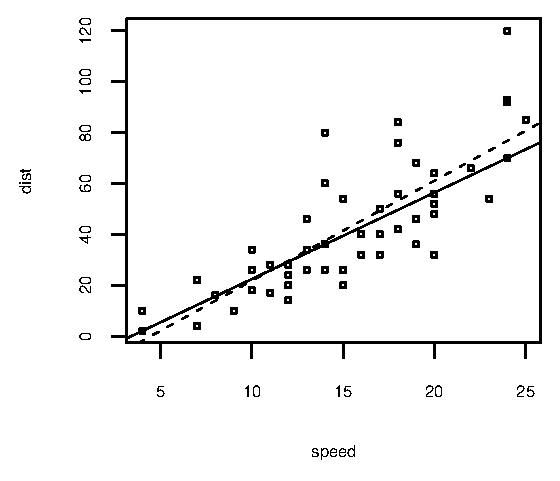
\includegraphics[height=50mm]{figures/fig12-05.eps}
\end{center}
Comparing a simple linear regression model (dashed line) for the `cars' data set with a support vector
regression model (solid line).
\es

\bs{Examples}
\vspace{.2in}
\begin{center}
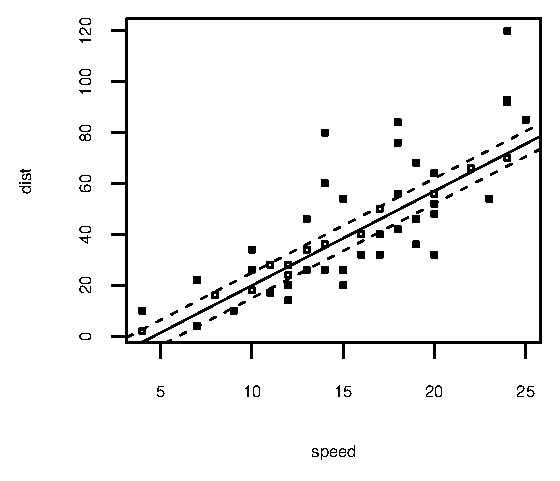
\includegraphics[height=40mm]{figures/fig12-06.eps}(a)
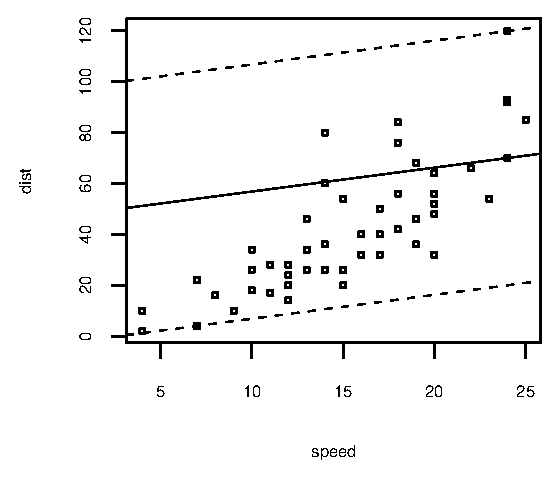
\includegraphics[height=40mm]{figures/fig12-07.eps}(b)
\end{center}
Linear support vector regression model of the `cars' data set with (a) $\varepsilon = 5$ and (b) $\varepsilon = 50$.
\es

\bs{Non-Linear Regression}
{\small
\begin{center}
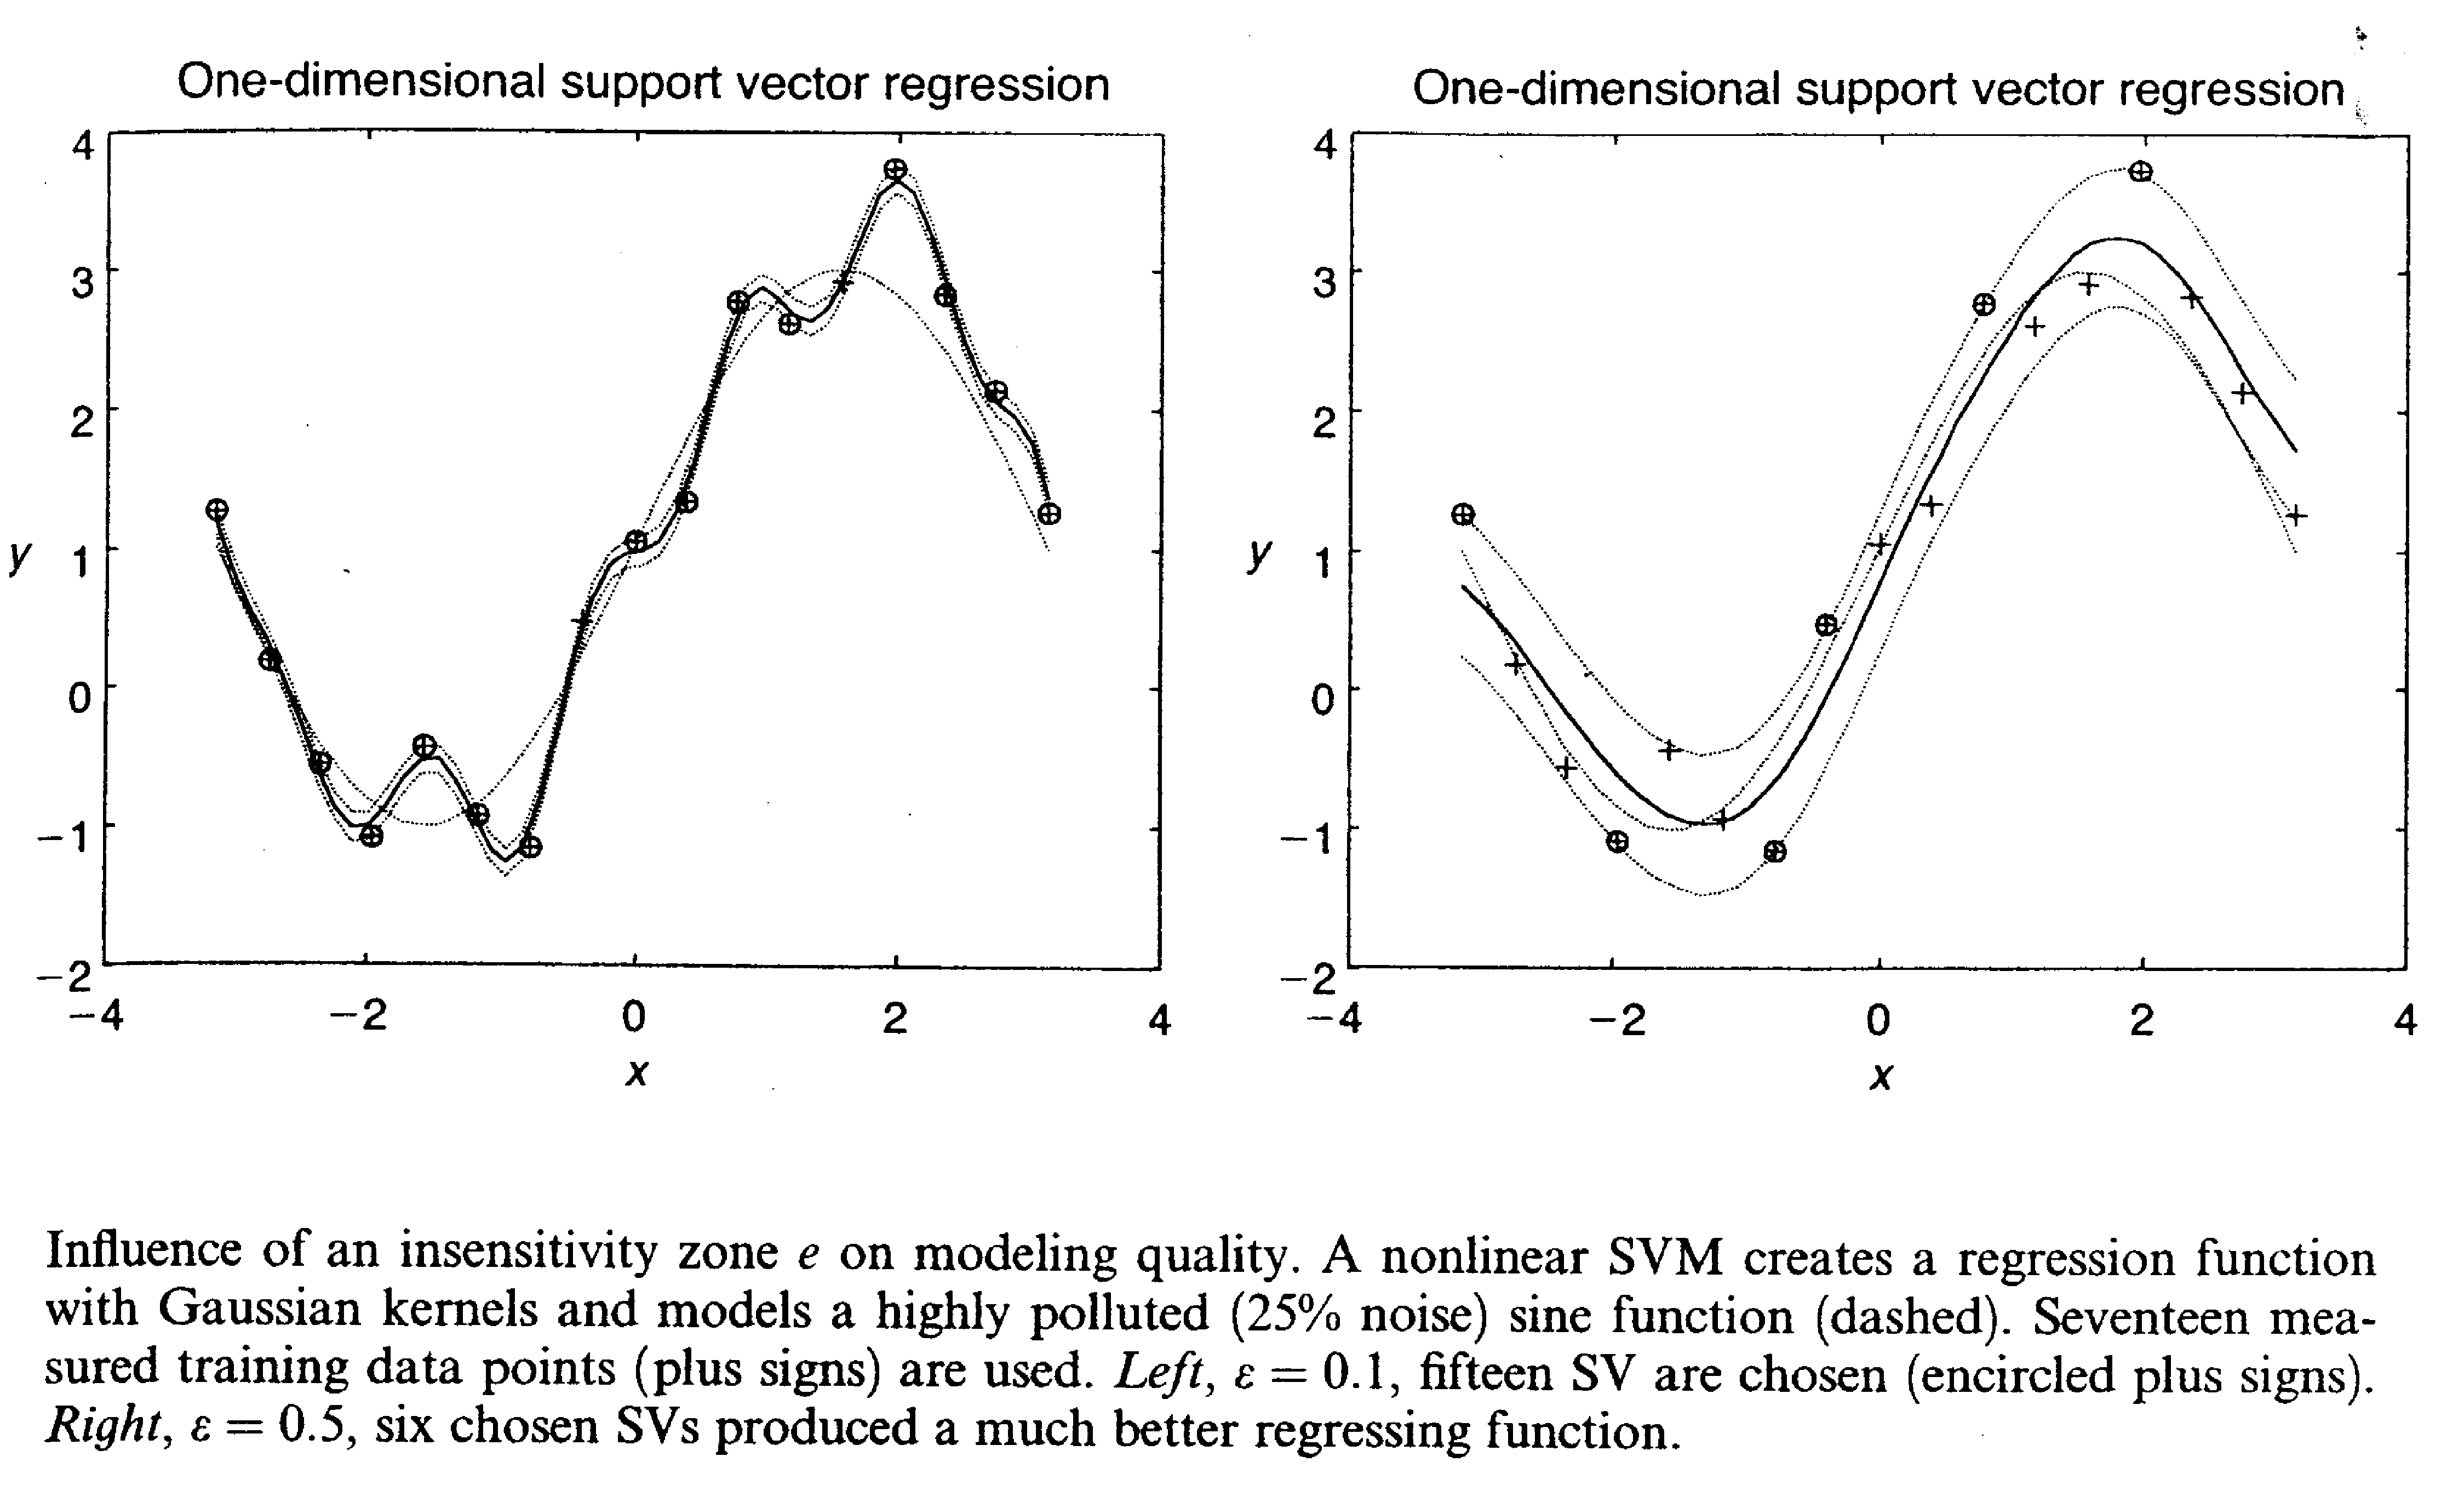
\includegraphics[height=60mm]{figures/nonlinear-regression.eps}
\end{center}

(Source: Learning and Soft Computing, V. Kecman, MIT Press, 2001)
}
\es

\end{document}
%%%%%%%%%%%%%%%%%%%%%%%%%%% end of template1.tex %%%%%%%%%%%%%%%%%%%%%%%%%%%%%%%%

